\documentclass{beamer}
\usepackage{times}
\usepackage{tikz}
\usepackage{beamerthemesplit}
\usetheme{Antibes}
\usepackage{tcolorbox}

\title{The Security Framework of White-Box Cryptography Revisited}
\author{Tao Sun, Yufeng Tang, Zheng Gong\\ \url{cis.gong@gmail.com}}
\institute{\inst{1}{School of Computer Science, South China Normal University} \\ \inst{2}{Mobile Applications And Security Engineering Center of Guangdong Province}}

\date{\today}

\begin{document}

\frame
{
 \titlepage
}

\section[Outline]{}
\frame{\tableofcontents}

\section{White-box cryptography: background}
\frame{
\frametitle{Cryptography: the very beginning}
"Information theory is about communication in the presence of noise."
\begin{flushright}
-C. Shannon, 1948.\footnote{\scriptsize{\url{http://fab.cba.mit.edu/classes/S62.12/docs/Shannon_noise.pdf}}}
\end{flushright}

\begin{center}
\begin{tikzpicture}
    \node[anchor=south west,inner sep=0] (image) at (0,0) { 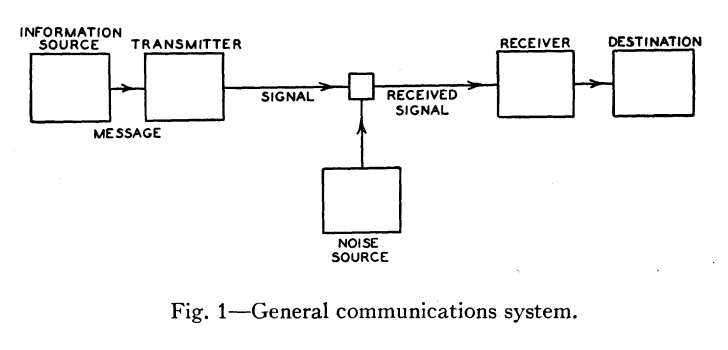
\includegraphics[width=8cm, height=4cm]{./pics/Shannon_GeneralCommunicationSystem.png}};

    %\begin{scope}[x={(image.south east)},y={(image.north west)}]
        %\draw[help lines,xstep=.1,ystep=.1] (0,0) grid (1,1);
        %\foreach \x in {0,1,...,9} { \node [anchor=north] at (\x/10,0) {0.\x}; }
        %\foreach \y in {0,1,...,9} { \node [anchor=east] at (0,\y/10) {0.\y}; }
        %\draw[green, ultra thick, rounded corners] (0.24,0.18) rectangle (0.50,0.32);
    %\end{scope}
\end{tikzpicture}
\end{center}
}

\frame{
\frametitle{Cryptography: an informal definition}
"Cryptography is about communication in the presence of adversaries."
\begin{flushright}
-R. Rivest
\end{flushright}

\begin{center}
\begin{tikzpicture}
    \node[anchor=south west,inner sep=0] (image) at (0,0) { 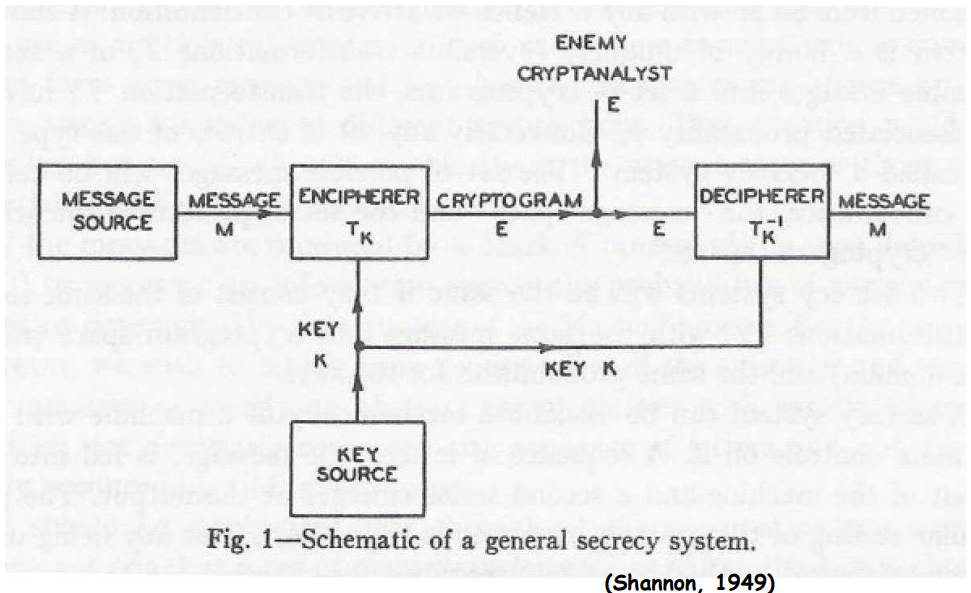
\includegraphics[width=8cm, height=5cm]{./pics/Shannon_GeneralSecrecySystem.png}};

    %\begin{scope}[x={(image.south east)},y={(image.north west)}]
        %\draw[help lines,xstep=.1,ystep=.1] (0,0) grid (1,1);
        %\foreach \x in {0,1,...,9} { \node [anchor=north] at (\x/10,0) {0.\x}; }
        %\foreach \y in {0,1,...,9} { \node [anchor=east] at (0,\y/10) {0.\y}; }
        %\draw[green, ultra thick, rounded corners] (0.24,0.18) rectangle (0.50,0.32);
    %\end{scope}
\end{tikzpicture}
\end{center}
}

\frame{
\frametitle{Define a secrecy system in ``a mathematically acceptable way"}
\textcolor{red}{``As a first step in the mathematical analysis of cryptography, it is necessary to idealize the situation suitably, and to define in a mathematically acceptable way what we shall mean by a secrecy system."}

\begin{flushright}
-C. Shannon, 1949. \footnote{{\scriptsize``Communication Theory of Secrecy Systems", Bell System Tech. J., vol. 28, pp. 656-715, Oct., 1949.}}
\end{flushright}
}

\frame{
\frametitle{The Kerckhoffs' principle of a secrecy system}
A cipher should be secure when the enemy cryptanalyst knows all details of the enciphering process and deciphering process except for the value of the secret key.

\begin{flushright}
- stated in 1881 by the Dutchman Auguste Kerckhoffs (1835-1903).
\end{flushright}


\begin{center}
\begin{tikzpicture}
    \node[anchor=south west,inner sep=0] (image) at (0,0) { 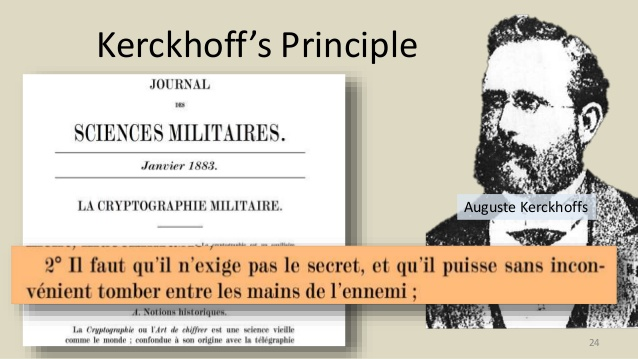
\includegraphics[width=6cm, height=4cm]{./pics/Kerckhoffs.jpg}};

    %\begin{scope}[x={(image.south east)},y={(image.north west)}]
        %\draw[help lines,xstep=.1,ystep=.1] (0,0) grid (1,1);
        %\foreach \x in {0,1,...,9} { \node [anchor=north] at (\x/10,0) {0.\x}; }
        %\foreach \y in {0,1,...,9} { \node [anchor=east] at (0,\y/10) {0.\y}; }
        %\draw[green, ultra thick, rounded corners] (0.24,0.18) rectangle (0.50,0.32);
    %\end{scope}
\end{tikzpicture}
\end{center}
}

\frame{
\frametitle{The goal of modern cryptography}
\begin{itemize}
\item The goal of modern cryptography is to design, analysis, and implement a secrecy system which obtains a mathematically acceptable security proofs.

\begin{itemize}
\item Confidentiality / Secrecy
\item Integrity
\item Authenticity
\item Availability
\end{itemize}

\item Thus provable security must be reduced on \textcolor{red}{an acceptable model!}
\begin{itemize}
\item Ideal cipher model
\item Random oracle model
\item Indifferentiability model
\end{itemize}
\end{itemize}
}

\frame{
\frametitle{How to modeling attackers in cryptography}
\begin{center}
\begin{tikzpicture}
    %\node[anchor=south west,inner sep=0] (image) at (0,0) { 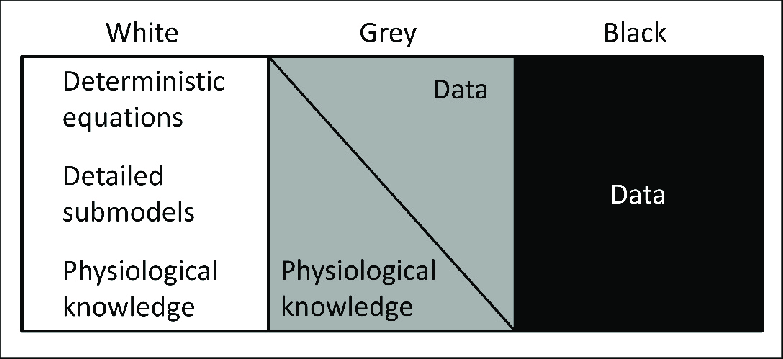
\includegraphics[width=6cm, height=4cm]{./pics/Illustration-of-the-concept-of-Black-White-Grey-box-modeling.png}};
    \node[anchor=south west,inner sep=0] (image) at (0,0) { 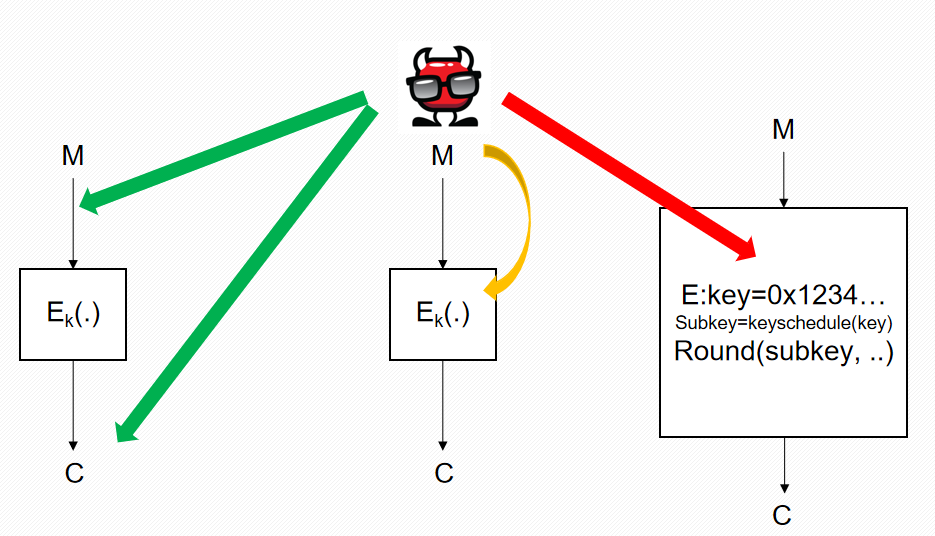
\includegraphics[width=7cm, height=4cm]{./pics/WBC_Model.png}};

    %\begin{scope}[x={(image.south east)},y={(image.north west)}]
        %\draw[help lines,xstep=.1,ystep=.1] (0,0) grid (1,1);
        %\foreach \x in {0,1,...,9} { \node [anchor=north] at (\x/10,0) {0.\x}; }
        %\foreach \y in {0,1,...,9} { \node [anchor=east] at (0,\y/10) {0.\y}; }
        %\draw[green, ultra thick, rounded corners] (0.24,0.18) rectangle (0.50,0.32);
    %\end{scope}
\end{tikzpicture}
\end{center}
}

\section{The security framework of WBC}
\subsection{Basic concepts of modeling}
\frame{
\frametitle{Black-box model}
\begin{itemize}
\item The adversary is able to know, choose or adaptively choose inputs and outputs of the function. 

\item Given the black-box implementation of the function, the adversary aims to \textcolor{red}{recover the secret values} or to \textcolor{orange}{misbehave the function}.
\end{itemize}
}

\frame{
\frametitle{White-box model}
\begin{itemize}
\item Informally speaking, an adversary in \textcolor{red}{white-box model} can tamper, modify, manipulate all intermediate values and processes of the implementation of a secrecy system.
\item It can be looked as a superset of \textcolor{red}{black-box} and \textcolor{red}{grey-box} models.
\end{itemize}
}

\frame{
\frametitle{Grey-box model}
According to the black/white-box modeling, the grey-box adversary is able to
\begin{itemize}
\item know, choose or adaptively choose inputs and outputs of the function;

\item tamper, modify, manipulate intermediate values with specific (physical) knowledge.

\end{itemize}
}

\frame{
\frametitle{An illustration of the Black/White/Grey-box modeling}
\begin{center}
\begin{tikzpicture}
    \node[anchor=south west,inner sep=0] (image) at (0,0) { 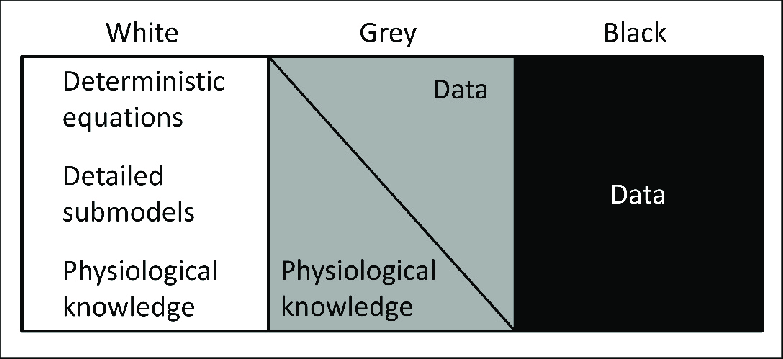
\includegraphics[width=9cm, height=4cm]{./pics/Illustration-of-the-concept-of-Black-White-Grey-box-modeling.png}};
    %\node[anchor=south west,inner sep=0] (image) at (0,0) { 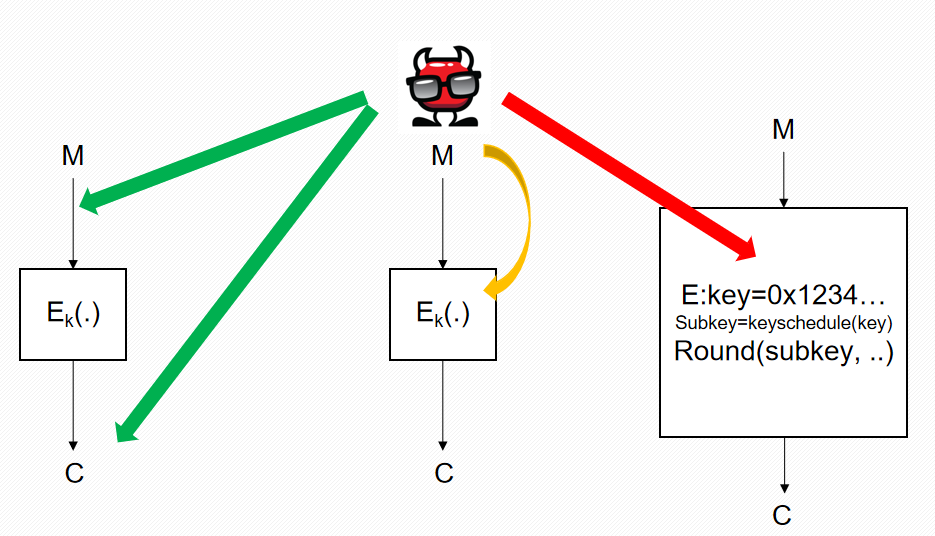
\includegraphics[width=7cm, height=4cm]{./pics/WBC_Model.png}};

    %\begin{scope}[x={(image.south east)},y={(image.north west)}]
        %\draw[help lines,xstep=.1,ystep=.1] (0,0) grid (1,1);
        %\foreach \x in {0,1,...,9} { \node [anchor=north] at (\x/10,0) {0.\x}; }
        %\foreach \y in {0,1,...,9} { \node [anchor=east] at (0,\y/10) {0.\y}; }
        %\draw[green, ultra thick, rounded corners] (0.24,0.18) rectangle (0.50,0.32);
    %\end{scope}
\end{tikzpicture}
\end{center}
}

\subsection{The proposed security notions and their problems}

\frame{
\frametitle{Chow \textit{et al.}'s definitions}
In Chow \textit{et al.}'s seminal work on white-box AES implementations, they proposed some basic notions intuitively.
\begin{itemize}
\item White-box attack context
\item

\end{itemize}
}

\frame{
\frametitle{Basic security definitions for WBC}
\begin{definition}(\textcolor{red}{Secret key recovery (KR-Security)}). A white-box implementation of a key-instantiated block cipher $E_{k}$ (or $D_{k}$) is called \textit{KR-insecure} if an attacker extracts the secret key $k$ and furthermore has access to the plaintext $P$.
\end{definition}

\begin{definition}
(\textcolor{red}{White-box key recovery (WBKR-Security)}). A white-box implementation of an encoded version of a key-instantiated block cipher $E_{k}$ (or $D_{k}$) is called \textit{WBKR-insecure} if the attacker extracts the secret key $k$ and the inverse mappings of the applied external encodings.
\end{definition}
}

\frame{
\frametitle{Basic security definitions for WBC (Chow \textit{et al.})}
\begin{itemize}
\item In SAC 2002, the security notions have  been informally described for white-box cryptography by Chow \textit{et al.}. First the key recovery problem is informally defined by \textcolor{red}{the weak white-box security} (which equals to \textcolor{red}{KR-Security})
\end{itemize}

\begin{center}
\begin{tikzpicture}
    \node[anchor=south west,inner sep=0] (image) at (0,0) { 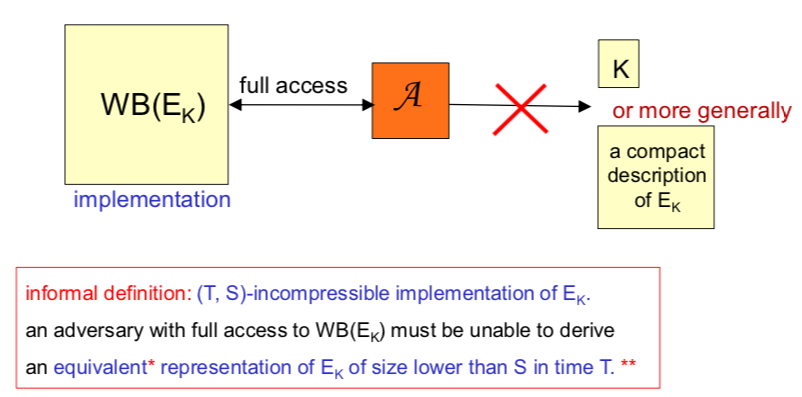
\includegraphics[width=8cm, height=4cm]{./pics/weak_white_box_security.png}};

    \begin{scope}[x={(image.south east)},y={(image.north west)}]
        %\draw[help lines,xstep=.1,ystep=.1] (0,0) grid (1,1);
        %\foreach \x in {0,1,...,9} { \node [anchor=north] at (\x/10,0) {0.\x}; }
        %\foreach \y in {0,1,...,9} { \node [anchor=east] at (0,\y/10) {0.\y}; }
        \draw[red, thin, rounded corners] (0.85,0.7) circle (1.2cm);
    \end{scope}
\end{tikzpicture}
\end{center}
}

\frame{
\frametitle{Basic security definitions for WBC (Biryukov \textit{et al.})}
\begin{itemize}
\item For more general security, \textcolor{red}{the strong white-box security} has been defined by [Biryukov \textit{et al.} 2014] (which connects to \textcolor{red}{KR/WBKR-Security})
\end{itemize}

\begin{center}
\begin{tikzpicture}
    \node[anchor=south west,inner sep=0] (image) at (0,0) { 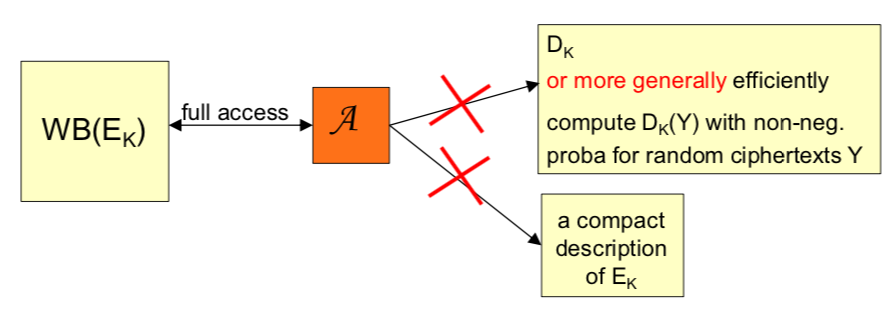
\includegraphics[width=10cm, height=4cm]{./pics/strong_white_box_security.png}};

    %\begin{scope}[x={(image.south east)},y={(image.north west)}]
        %\draw[help lines,xstep=.1,ystep=.1] (0,0) grid (1,1);
        %\foreach \x in {0,1,...,9} { \node [anchor=north] at (\x/10,0) {0.\x}; }
        %\foreach \y in {0,1,...,9} { \node [anchor=east] at (0,\y/10) {0.\y}; }
        %\draw[green, ultra thick, rounded corners] (0.24,0.18) rectangle (0.50,0.32);
    %\end{scope}
\end{tikzpicture}
\end{center}
}


\frame{
\frametitle{The problems of the weak/strong white-box security}
\begin{itemize}
\item It only works for white-box encryption/decryption, while does not suitable for \textcolor{red}{MAC/signature}.

\item ``A \textcolor{red}{compact} description of $E_{k}$/$/D_{k}$", it is very hard to measure security under this informal definition.
\end{itemize}
}

\frame{
\frametitle{The negative results on virtual black-box property (VBBP)}
\begin{itemize}
\item At Crypto 2001, Barak \textit{et al.} provided an insight on the impossibility of code obfuscation for \textcolor{red}{generic programs}.
\item \textcolor{red}{The virtual black-box property (VBBP)} has been proposed for defining the ideal code/program obfuscation.
\item The negative results are given by counterexamples that cannot satisfy the virtual black-box property (VBBP) in any circumstance.
\end{itemize}
}

\frame{
\frametitle{Recall the definitions of VBBP [Saxena2009] (1)}
\textbf{Correctness.}{$\mathcal{O}$ is an obfuscator for a polynomial time function $Q$ if the follow properties hold.}
\begin{enumerate}

\item \textit{(\textcolor{red}{Functionality})}. $\forall k, \forall (q,a)\in \mathcal{K}^{k}_{Q}\times \mathcal{I}^{k}_{Q}:\textmd{Pr}[\mathcal{O}(Q,k)(a) \neq Q [k](a)]\leq negl(k)$

\item \textit{(\textcolor{red}{Polynomial slowdown and expansion})}. $\exists p \in \mathbb{P}, \forall k, \forall q \in \mathcal{K}^{k}_{Q}:$
\begin{itemize}
    \item $|\mathcal{O}(Q, q)| \leq p(k)$;
    \newline
    \item $\forall a: Q[q](a) \leq t \rightarrow \mathcal{O}(Q,q)(a) \leq p(t)$
\end{itemize}
\end{enumerate}
}

\frame{
\frametitle{Recall the definitions of VBBP [Saxena2009] (2)}
\begin{itemize}
\item Let $Q[q]$ be a random instance of a polynomial Turing machine family (PTMF) $Q$ under key $q$.

\item The VBBP requires that whatever information that adversary $\mathcal{A}$ extracts from $\mathcal{O}(Q,q)$, simulator $\mathcal{S}$ can also extract with black-box access to $Q[q]$.

\item The existing notions of VBBP can be categorized in the following two directions.
\begin{itemize}
\item \textit{Predicate VBBP}

\item \textit{Indistinguishability}
\end{itemize}

\end{itemize}

[Saxena 2009] noted that \textit{Predicate VBBP(pvbbp)} is too weak for practice, on the other hand \textit{Indistinguishability} is too strong to be achievable.
}

\frame{
\frametitle{Recall the definitions of VBBP [Saxena2009] (3)}

\textbf{Soundness.}{$\mathcal{O}$ is sound if at least one of the following properties holds.}
\begin{enumerate}
\item \textit{Predicate VBBP:}$\forall A\in \mathbb{PPT}, \exists S \in \mathbb{PPT}: Adv_{A, S, \mathcal{O}, Q}^{pvbbp} \leq negl(k)$, where \\ $Adv_{A, S, \mathcal{O}, Q}^{pvbbp}(k) =|\textmd{Pr}_{q \xleftarrow{R} \mathcal{K}^{k}_{Q}}[A^{Q[q]}(1^{k},\mathcal{O}(Q,q))=1 \wedge S^{Q[q]}(1^{k})\neq 1]|$.

\item \textit{Indistinguishability:} $\forall A\in \mathbb{PPT}, \exists S \in \mathbb{PPT}: Adv_{A, S, \mathcal{O}, Q}^{ind} \leq negl(k)$, where \\ $Adv_{A, S, \mathcal{O}, Q}^{ind}(k) =|\textmd{Pr}_{q \xleftarrow{R} \mathcal{K}^{k}_{Q}}[A^{Q[q]}(1^{k},\mathcal{O}(Q,q))=1 \wedge A^{Q[q]}(1^{k}, S^{Q[q]}(1^{k}))\neq 1]|$.
\end{enumerate}


}

\frame{
\frametitle{Saxena \textit{et al.}'s WBC proposal}
\begin{enumerate}
\item Encryption: $E[k]:(m, r) \mapsto (H(\hat{e}(\textcolor{red}{k}^{r}, g)\oplus m), g^{r}) \mapsto (c_{1}, c_{2})$

\item Decryption:$D[k]: (c_{1}, c_{2}) \mapsto H(\hat{e}(c_{2}, k))\oplus c_{1} \mapsto m$

\item White-box encryption: Let $y = \textcolor{red}{\hat{e}(k, g)}$, $\mathcal{O}(E[k]): (m, r) \mapsto (H( \textcolor{red}{y}^{r}) \oplus m, g^{r}) \mapsto (c_{1}, c_{2})$\newline

\end{enumerate}


The problem:
\begin{itemize}
\item only CPA-security, to achieve CCA-Security requires MAC on message. (\textcolor{red}{which means another authenticated key!})

\item Black-box security can be reduced to the discrete logarithm problem (\textcolor{red}{$k^{r}$}), whilst white-box security is the pairing inversion problem. ($y = \hat{e}(\textcolor{red}{k}, g)$)
\end{itemize}
}


\subsection{Application-oriented security notions}

\frame
{
\frametitle{Tamper resistance for DRM}

\begin{itemize}
\item Michiels and Gorissen [DRM'07] proposed a method to protect the integrity of software which depends on the correct operation of the white-box implementation of a block cipher.
%\item If an attacker modifies the software, the white-box implementation stops decrypting/encrypting properly.
\begin{tcolorbox}[title=security goal]
\item The proposed method assume that it is the goal of an attacker to \textcolor{red}{modify} the protected software without losing the ability to decrypt/encrypt properly.
\end{tcolorbox}
\end{itemize}

}

\frame{

\frametitle{White-box security objectives}
For the application in which a white-box implementation is deployed, [Delerabl$\acute{e}$e \textit{et al.} 2013] discussed the following security objectives.

\begin{itemize}
\item One-wayness: implies the strong white-box security

\item Incompressibility: prevents the a functionally equivalent deduction \textcolor{red}{with a significantly smaller memory footprint}.

\item Traceability: make a white-box implementation traceable.

\end{itemize}

}

\frame{
\frametitle{White-box metrics}
Chow \textit{et al.} [CEJO 2002] introduced a few metrics that try to measure the achieved level of white-box security for LUT-based implementations.
\begin{itemize}
\item White-box diversity

\item White-box ambiguity

\item local security
\end{itemize}
}

\frame{


}

\section{Our concerns on the security framework of WBC}

\frame{
\frametitle{The practical perspective of white-box security}
Under the definitions of the black-box and the white-box securities, we propose a practical perspective of the white-box cryptography. The perspective is depicted from what the white-box cryptography can provide and how it should be secure against the adversary. Since the secret values are the most important in the white-box security model. A white-box cryptography can provide the following security properties.

\begin{itemize}
\item \textbf{Algorithm level: \textcolor{red}{Key recovery}.}

\item \textbf{Module level: Function integrity.}

\item \textbf{System level: Code lifting}

\end{itemize}
}

\frame{
\frametitle{}
Based on the above security properties that white-box cryptography could provide, one can build up secure applications enjoys the white-box security. From the life-cycle of secret keys, we depict the typical usages of the white-box cryptography in the following ways.

\begin{itemize}
\item \textbf{Key distribution.} Normally, the applications need a secure channel to distribute the secret keys between server and client. Although some key distribution schemes can be executed under authenticated channel, but most of them still need the support of certification services (Such as PKI, PKG, etc.). Because the white-box cryptography protects the secret keys from the adversary, the distribution of the keys only requires authenticated channel. If

\item \textbf{Local key management.}

\item \textbf{Dynamic key updating.}

\item \textbf{Key revocation.}
\end{itemize}
}

\frame{
\frametitle{}
For symmetric-key algorithms, they might be used for message authentication, data encryption/decrypiton and pseudorandom number generating. According to these different usages, the security requirements for the implementations of those cryptographic algorithms are diverse. Considering this diversity, we define a practical security notion for white-box cryptography as follows.

\begin{itemize}
\item \textbf{Key integrity.}

\item \textbf{Key confidentiality.}

\item \textbf{Key equivalence.}
\end{itemize}

}

\section{Conclusion}

\frame
{
\frametitle{Conclusion}

\begin{itemize}
\setlength{\itemsep}{12pt}
\item Security notions and definition for \textcolor{red}{precisely} analyze white-box cryptography are at very beginning.

\item Key protection definitions might not suitable in practice for non-key white-box applications, e.g., secure multi-party computation.

\item A secure white-box cryptography does not imply the white-box security of a secrecy system based on it.
\end{itemize}

}

\frame
{
\begin{center}
\textbf{Thanks for your attentions!}
\end{center}
\begin{center}
\begin{tikzpicture}
    \node[anchor=south west,inner sep=0] (image) at (0,0) { 
\includegraphics[width=4cm, height=4cm]{./pics/WBC_BG.png}};

    %\begin{scope}[x={(image.south east)},y={(image.north west)}]
        %\draw[help lines,xstep=.1,ystep=.1] (0,0) grid (1,1);
        %\foreach \x in {0,1,...,9} { \node [anchor=north] at (\x/10,0) {0.\x}; }
        %\foreach \y in {0,1,...,9} { \node [anchor=east] at (0,\y/10) {0.\y}; }
        %\draw[green, ultra thick, rounded corners] (0.24,0.18) rectangle (0.50,0.32);
    %\end{scope}
\end{tikzpicture}

\end{center}
}


\end{document}
